\documentclass[11pt]{article}

\usepackage[margin=1.6cm, landscape]{geometry}
\usepackage{tikz}
\usetikzlibrary{positioning, arrows.meta, decorations.pathreplacing, calc}
\usepackage{amsmath, amssymb}
\pagestyle{empty}

\tikzset{
  box/.style={draw, rounded corners, align=center, minimum height=0.9cm, inner sep=7pt, font=\small},
  lab/.style={font=\scriptsize, text=black!60},
  arr/.style={-{Stealth[length=6pt]}, thick, black!55},
  pt/.style={draw, circle, inner sep=0pt, minimum size=7mm, font=\scriptsize},
  thinarr/.style={-{Stealth[length=4pt]}, black!45},
}

\newcommand{\schemetitle}[1]{
  \begin{center}{\LARGE\textbf{#1}}
\end{center}\vspace{0.5cm}}
\newcommand{\schemenote}[1]{\vspace{0.4cm}
  \begin{center}\footnotesize\color{black!65} #1
\end{center}}

\begin{document}

% ============================================================
\schemetitle{1. Non-parametric (case) bootstrap}
\begin{center}
  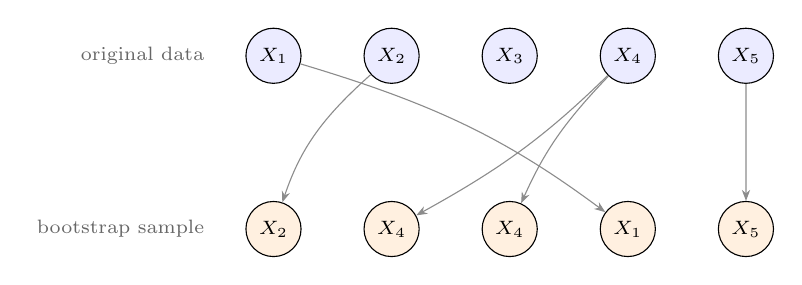
\begin{tikzpicture}[xscale=1.5]
    \node[pt, fill=blue!8] (o1) at (0,0) {$X_1$};
    \node[pt, fill=blue!8] (o2) at (1,0) {$X_2$};
    \node[pt, fill=blue!8] (o3) at (2,0) {$X_3$};
    \node[pt, fill=blue!8] (o4) at (3,0) {$X_4$};
    \node[pt, fill=blue!8] (o5) at (4,0) {$X_5$};
    \node[lab, left=0.4cm of o1] {original data};

    \node[pt, fill=orange!12] (b1) at (0,-2.2) {$X_2$};
    \node[pt, fill=orange!12] (b2) at (1,-2.2) {$X_4$};
    \node[pt, fill=orange!12] (b3) at (2,-2.2) {$X_4$};
    \node[pt, fill=orange!12] (b4) at (3,-2.2) {$X_1$};
    \node[pt, fill=orange!12] (b5) at (4,-2.2) {$X_5$};
    \node[lab, left=0.4cm of b1] {bootstrap sample};

    \draw[thinarr] (o2) to[bend right=12] (b1);
    \draw[thinarr] (o4) to[bend left=8]  (b2);
    \draw[thinarr] (o4) to[bend right=8] (b3);
    \draw[thinarr] (o1) to[bend left=12] (b4);
    \draw[thinarr] (o5) to (b5);
  \end{tikzpicture}
\end{center}
\schemenote{Each $X_i^{*}$ drawn independently and uniformly from $\{X_1,\dots,X_n\}$, with replacement.\\ $X_4$ gets picked twice, $X_3$ not at all --- typical of a single resample.}
\newpage

% ============================================================
\schemetitle{2. Parametric bootstrap}
\begin{center}
  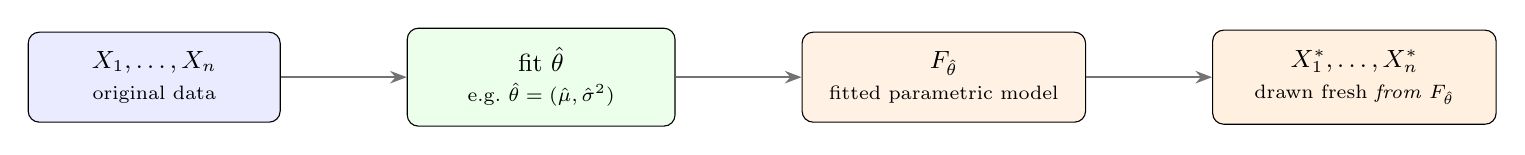
\begin{tikzpicture}[node distance=1.6cm]
    \node[box, fill=blue!8, minimum width=3.2cm] (data) {$X_1,\dots,X_n$ \\ \scriptsize original data};
    \node[box, fill=green!8, minimum width=3.4cm, right=of data] (fit) {fit $\hat\theta$ \\ \scriptsize e.g.\ $\hat\theta=(\hat\mu,\hat\sigma^2)$};
    \node[box, fill=orange!10, minimum width=3.6cm, right=of fit] (model) {$F_{\hat\theta}$ \\ \scriptsize fitted parametric model};
    \node[box, fill=orange!12, minimum width=3.6cm, right=of model] (boot) {$X_1^{*},\dots,X_n^{*}$ \\ \scriptsize drawn fresh \emph{from $F_{\hat\theta}$}};

    \draw[arr] (data) -- (fit);
    \draw[arr] (fit) -- (model);
    \draw[arr] (model) -- (boot);
  \end{tikzpicture}
\end{center}
\schemenote{The bootstrap sample never touches the raw data again --- it comes entirely from the fitted model.\\ Good only as far as the parametric assumption is right.}
\newpage

% ============================================================
\schemetitle{3. Residual bootstrap (regression)}
\begin{center}
  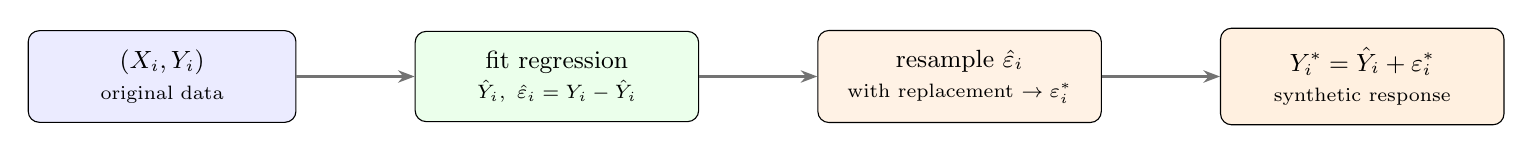
\begin{tikzpicture}[node distance=1.5cm]
    \node[box, fill=blue!8, minimum width=3.4cm] (data) {$(X_i, Y_i)$ \\ \scriptsize original data};
    \node[box, fill=green!8, minimum width=3.6cm, right=of data] (fit) {fit regression \\ \scriptsize $\hat Y_i,\ \hat\varepsilon_i = Y_i - \hat Y_i$};
    \node[box, fill=orange!10, minimum width=3.6cm, right=of fit] (resample) {resample $\hat\varepsilon_i$ \\ \scriptsize with replacement $\to \varepsilon_i^{*}$};
    \node[box, fill=orange!12, minimum width=3.6cm, right=of resample] (boot) {$Y_i^{*} = \hat Y_i + \varepsilon_i^{*}$ \\ \scriptsize synthetic response};

    \draw[arr] (data) -- (fit);
    \draw[arr] (fit) -- (resample);
    \draw[arr] (resample) -- (boot);
  \end{tikzpicture}
\end{center}
\schemenote{Residuals are shuffled \emph{across} observations --- assumes they're roughly exchangeable (homoscedastic).}
\newpage

% ============================================================
\schemetitle{4. Wild bootstrap}
\begin{center}
  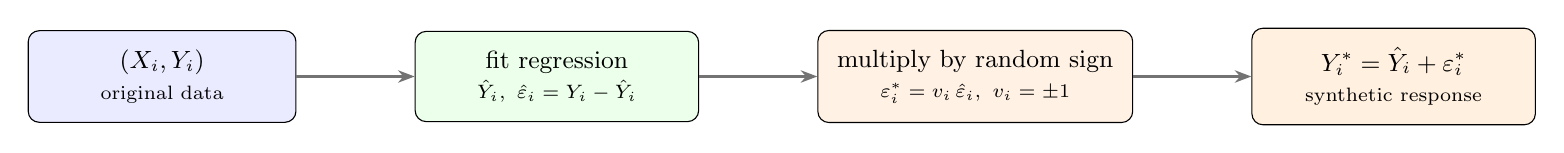
\begin{tikzpicture}[node distance=1.5cm]
    \node[box, fill=blue!8, minimum width=3.4cm] (data) {$(X_i, Y_i)$ \\ \scriptsize original data};
    \node[box, fill=green!8, minimum width=3.6cm, right=of data] (fit) {fit regression \\ \scriptsize $\hat Y_i,\ \hat\varepsilon_i = Y_i - \hat Y_i$};
    \node[box, fill=orange!10, minimum width=3.8cm, right=of fit] (weight) {multiply by random sign \\ \scriptsize $\varepsilon_i^{*} = v_i\,\hat\varepsilon_i,\ v_i=\pm1$};
    \node[box, fill=orange!12, minimum width=3.6cm, right=of weight] (boot) {$Y_i^{*} = \hat Y_i + \varepsilon_i^{*}$ \\ \scriptsize synthetic response};

    \draw[arr] (data) -- (fit);
    \draw[arr] (fit) -- (weight);
    \draw[arr] (weight) -- (boot);
  \end{tikzpicture}
\end{center}
\schemenote{Each residual stays attached to \emph{its own} observation $i$ --- only its sign is randomized.\\ Survives heteroscedasticity, where residual bootstrap (\S3) breaks.}
\newpage

% ============================================================
\schemetitle{5. Block bootstrap}
\begin{center}
  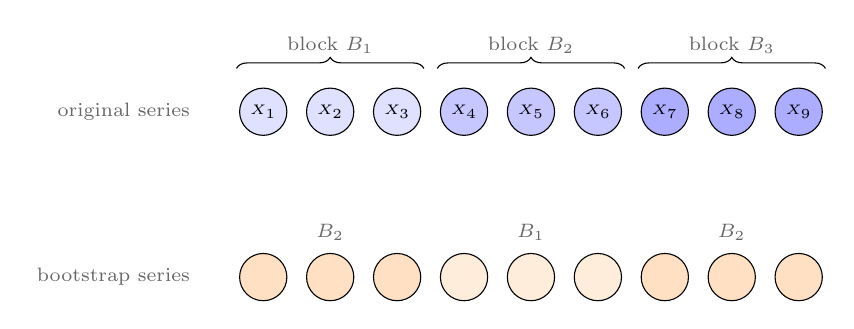
\begin{tikzpicture}[xscale=0.85]
    \foreach \i/\v/\col in {0/X_1/blue!12,1/X_2/blue!12,2/X_3/blue!12,3/X_4/blue!22,4/X_5/blue!22,5/X_6/blue!22,6/X_7/blue!32,7/X_8/blue!32,8/X_9/blue!32}{
      \node[pt, fill=\col, minimum size=6mm] (o\i) at (\i,0) {\tiny $\v$};
    }
    \draw[decorate, decoration={brace, amplitude=4pt}] (-0.4,0.55) -- (2.4,0.55) node[midway, above=2pt, lab] {block $B_1$};
    \draw[decorate, decoration={brace, amplitude=4pt}] (2.6,0.55) -- (5.4,0.55) node[midway, above=2pt, lab] {block $B_2$};
    \draw[decorate, decoration={brace, amplitude=4pt}] (5.6,0.55) -- (8.4,0.55) node[midway, above=2pt, lab] {block $B_3$};
    \node[lab, left=0.5cm of o0] {original series};

    \foreach \i/\col in {0/orange!24,1/orange!24,2/orange!24,3/orange!14,4/orange!14,5/orange!14,6/orange!24,7/orange!24,8/orange!24}{
      \node[pt, fill=\col, minimum size=6mm] (b\i) at (\i,-2.1) {};
    }
    \node[lab, left=0.5cm of b0] (blab) {bootstrap series};
    \node[lab, above=1pt of b1] {$B_2$};
    \node[lab, above=1pt of b4] {$B_1$};
    \node[lab, above=1pt of b7] {$B_2$};
  \end{tikzpicture}
\end{center}
\schemenote{Whole contiguous blocks of length $\ell$ (here $\ell=3$) are resampled with replacement, then concatenated.\\ Keeps short-range dependence \emph{inside} a block; sensitive to the choice of $\ell$.}
\newpage

% ============================================================
\schemetitle{6. Stationary bootstrap}
\begin{center}
  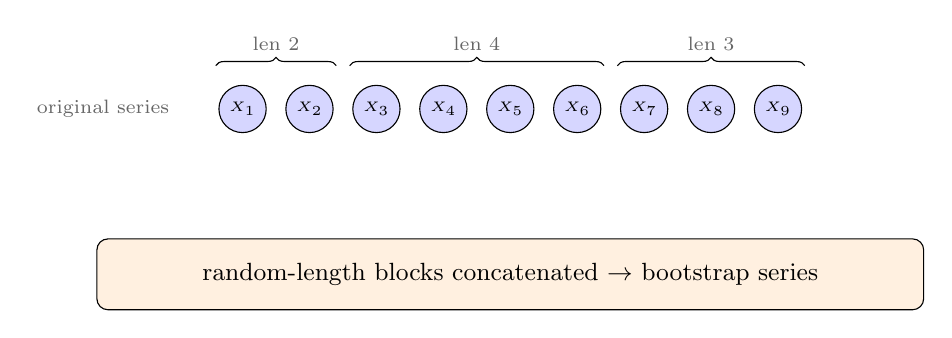
\begin{tikzpicture}[xscale=0.85]
    \foreach \i/\v in {0/X_1,1/X_2,2/X_3,3/X_4,4/X_5,5/X_6,6/X_7,7/X_8,8/X_9}{
      \node[pt, fill=blue!16, minimum size=6mm] (o\i) at (\i,0) {\tiny $\v$};
    }
    \node[lab, left=0.5cm of o0] {original series};

    \draw[decorate, decoration={brace, amplitude=3pt}] (-0.4,0.55) -- (1.4,0.55) node[midway, above=2pt, lab] {\scriptsize len 2};
    \draw[decorate, decoration={brace, amplitude=3pt}] (1.6,0.55) -- (5.4,0.55) node[midway, above=2pt, lab] {\scriptsize len 4};
    \draw[decorate, decoration={brace, amplitude=3pt}] (5.6,0.55) -- (8.4,0.55) node[midway, above=2pt, lab] {\scriptsize len 3};

    \node[box, fill=orange!12, minimum width=10.5cm, minimum height=0.9cm] (boot) at (4,-2.1) {random-length blocks concatenated $\to$ bootstrap series};
  \end{tikzpicture}
\end{center}
\schemenote{Same idea as block bootstrap, but block length is itself random (geometric distribution) instead of a fixed $\ell$.\\ Result doesn't hinge on one arbitrary block-length choice.}
\newpage

% ============================================================
\schemetitle{7. Bayesian bootstrap}
\begin{center}
  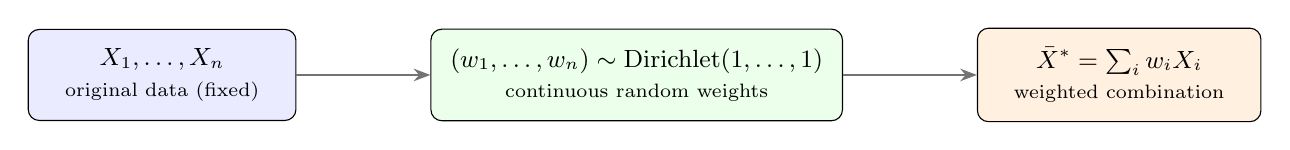
\begin{tikzpicture}[node distance=1.7cm]
    \node[box, fill=blue!8, minimum width=3.4cm] (data) {$X_1,\dots,X_n$ \\ \scriptsize original data (fixed)};
    \node[box, fill=green!8, minimum width=4.2cm, right=of data] (weights) {$(w_1,\dots,w_n)\sim\mathrm{Dirichlet}(1,\dots,1)$ \\ \scriptsize continuous random weights};
    \node[box, fill=orange!12, minimum width=3.6cm, right=of weights] (boot) {$\bar X^{*} = \sum_i w_i X_i$ \\ \scriptsize weighted combination};

    \draw[arr] (data) -- (weights);
    \draw[arr] (weights) -- (boot);
  \end{tikzpicture}
\end{center}
\schemenote{No resampling, no repeated points --- every observation is always used, just reweighted.\\ Smoother than the classic bootstrap; a Bayesian-flavored uncertainty estimate.}
\newpage

% ============================================================
\schemetitle{8. Smoothed bootstrap}
\begin{center}
  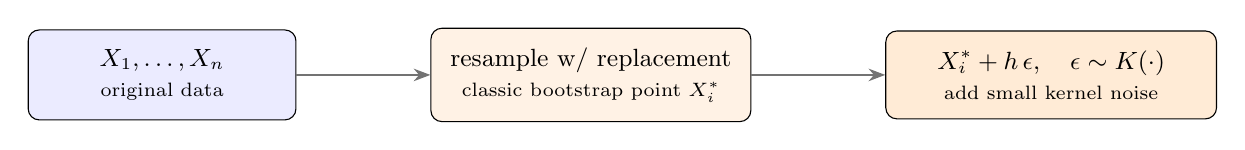
\begin{tikzpicture}[node distance=1.7cm]
    \node[box, fill=blue!8, minimum width=3.4cm] (data) {$X_1,\dots,X_n$ \\ \scriptsize original data};
    \node[box, fill=orange!10, minimum width=3.6cm, right=of data] (resample) {resample w/ replacement \\ \scriptsize classic bootstrap point $X_i^{*}$};
    \node[box, fill=orange!16, minimum width=4.2cm, right=of resample] (smooth) {$X_i^{*} + h\,\epsilon,\quad \epsilon\sim K(\cdot)$ \\ \scriptsize add small kernel noise};

    \draw[arr] (data) -- (resample);
    \draw[arr] (resample) -- (smooth);
  \end{tikzpicture}
\end{center}
\schemenote{A touch of noise smooths out the ``lumpy'', discrete look of the raw empirical distribution.\\ Useful when the statistic is sensitive to exact ties or discreteness.}
\newpage

% ============================================================
\schemetitle{9. $m$-out-of-$n$ bootstrap / subsampling}
\begin{center}
  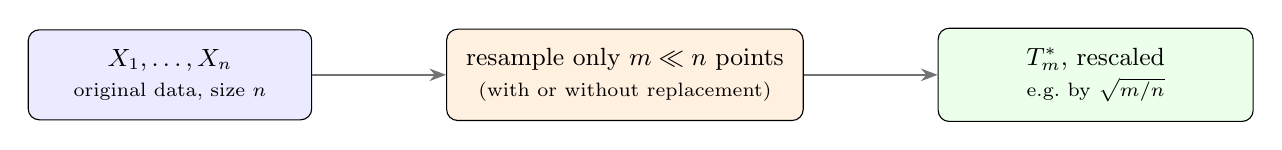
\begin{tikzpicture}[node distance=1.7cm]
    \node[box, fill=blue!8, minimum width=3.6cm] (data) {$X_1,\dots,X_n$ \\ \scriptsize original data, size $n$};
    \node[box, fill=orange!12, minimum width=3.8cm, right=of data] (resample) {resample only $m \ll n$ points \\ \scriptsize (with or without replacement)};
    \node[box, fill=green!8, minimum width=4.0cm, right=of resample] (boot) {$T_m^{*}$, rescaled \\ \scriptsize e.g.\ by $\sqrt{m/n}$};

    \draw[arr] (data) -- (resample);
    \draw[arr] (resample) -- (boot);
  \end{tikzpicture}
\end{center}
\schemenote{A smaller resample means a lower chance of re-selecting the same extreme point every time.\\ Fixes the failure mode of \S1 for statistics like the sample min/max --- at the cost of choosing $m$.}

\end{document}
